\documentclass[11pt,a4paper]{ctexart}

\usepackage[a4paper,margin=2.4cm]{geometry}
\usepackage{graphicx}
\usepackage{xcolor}
\usepackage{caption}
\usepackage{enumitem}
\usepackage{amsmath,amssymb}
\usepackage{booktabs}
\usepackage[hidelinks]{hyperref}

\captionsetup{font=small,labelfont=bf}
\setlist{nosep}

% 审稿人问题环境：引用缩进 + 灰色英文原文（仅用基础包）
\newcommand{\reviewer}[1]{\par\medskip\begin{quote}\small\color{gray!70!black}%
  \textbf{审稿人意见（原文）：}#1\end{quote}\medskip}
\newcommand{\response}{\par\medskip\textbf{回复：}}

\title{\bfseries 回复信：第一位审稿人\\[4pt]\large 逐条回复与修改说明}
\author{}
\date{}

\begin{document}

\maketitle

感谢审稿人仔细阅读我们的稿件，并提出深刻而有帮助的意见。这些意见显著提高了
我们工作的质量。以下逐条回复；所有修改已在修改稿中高亮标出，图表与参考文献
均已相应更新。

\section*{第 1 条 —— 选择固体的动机、与气体研究的关系}

\reviewer{It is not clear to me what is the motivation for using a solid, and what
are the differences with respect to the typical gas phase. The authors cite some
works of HHG beyond the dipole approximation in gases, some even using vortex beams
too, and they state that this interaction has not been explored in solids. Thus,
what is the relation of this work with the existing studies using gases? Do they
find the same OAM selection rules for the even harmonics (equation 1)? Have the
present selection rules been observed/computed before? Which is the role of the
solid here with respect to a gas? This information would help put the work into
context and have a broader understanding of the topic of study.}

\response 选择固体靶材的动机是让\textbf{双靶材干涉}方案切实可行。气体因扩散
特性难以把两个发射体固定在确定的方位角位置（例如 $0^\circ$ 和 $90^\circ$）；
而固体样品可以自然、可重复地固定在任意面内取向，这正是双靶材干涉几何所
需要的。

按照审稿人的建议，我们完成了对应的气体计算，结果非常好，显著提升了工作质量。
是的——\textbf{我们在气体中得到了与固体完全相同的 OAM 选择定则}：奇次谐波
$L=q\ell$，偶次谐波 $L=q\ell\pm1$（见新图 \ref{fig:gas_oam}）。值得注意的是，
在气体中只需一组工程上完全可行的参数（氢原子、SG1、1100 nm），偶次通道就已
经非常干净，甚至不需要双靶材干涉（新图 \ref{fig:gas_hhg}）。顺着审稿人的气体
思路，我们还合成了阿秒脉冲：相比固体，气体更适合产生阿秒脉冲，脉宽更短
（新图 \ref{fig:attosecond}）。这些结果已写入新增的``气体 HHG''章节。

\begin{figure}[htbp]
  \centering
  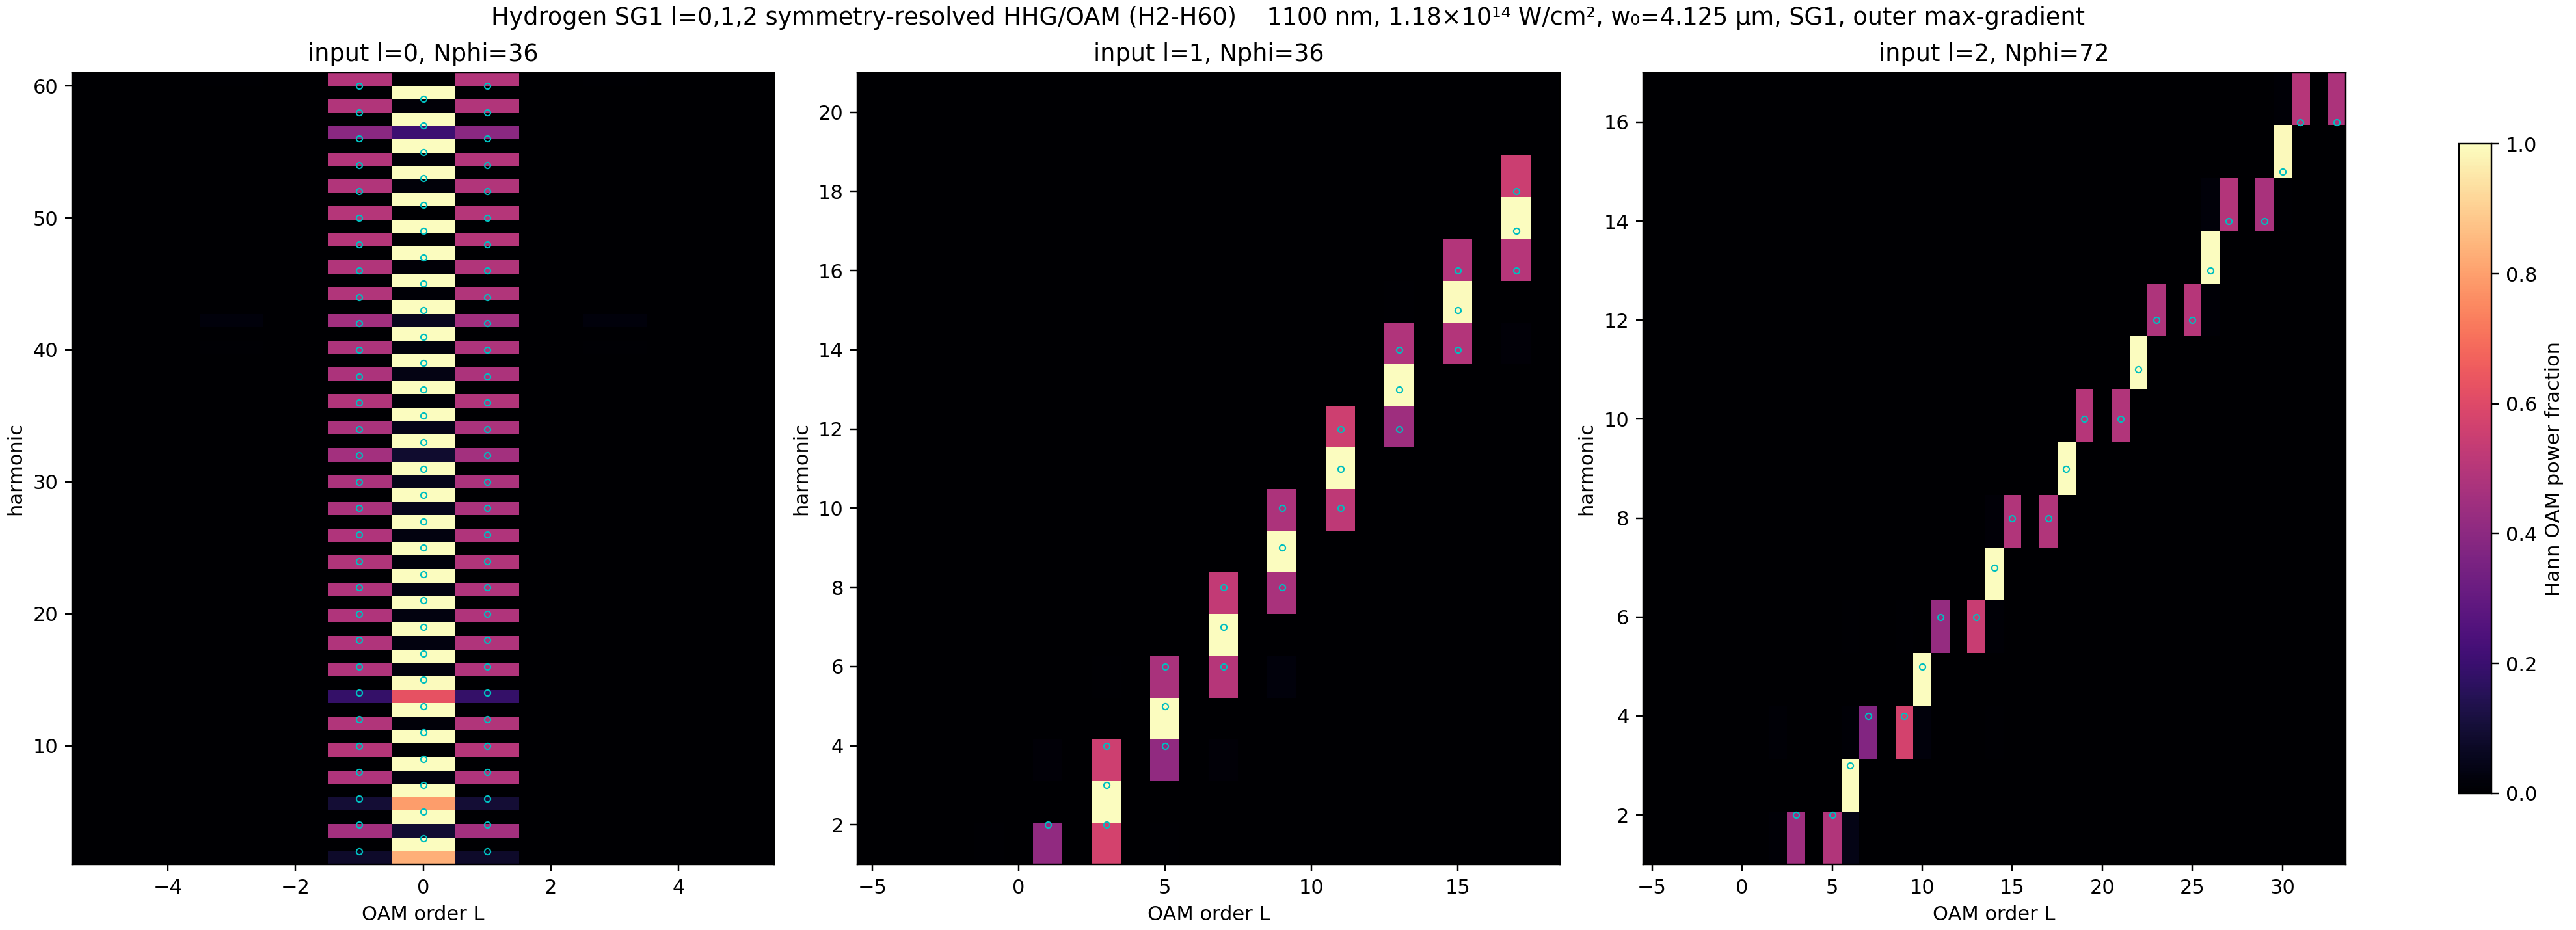
\includegraphics[width=0.98\linewidth]{reviewer_response_R1_figs/fig2_gas_oam.png}
  \caption{氢原子（SG1、1100 nm）144 角 OAM 分析：奇次 $L=q\ell$、偶次
  $L=q\ell\pm1$，与固体结果一致。子图显示范围（a）l=0：0--60 阶，
  （b）l=1：0--20 阶，（c）l=2：0--16 阶。OAM 轴限制在角度采样奈奎斯特
  范围内（l=0,1 为 36 角 $\Rightarrow |L|\le 18$；l=2 为 72 角
  $\Rightarrow |L|\le 36$）。}
  \label{fig:gas_oam}
\end{figure}

\begin{figure}[htbp]
  \centering
  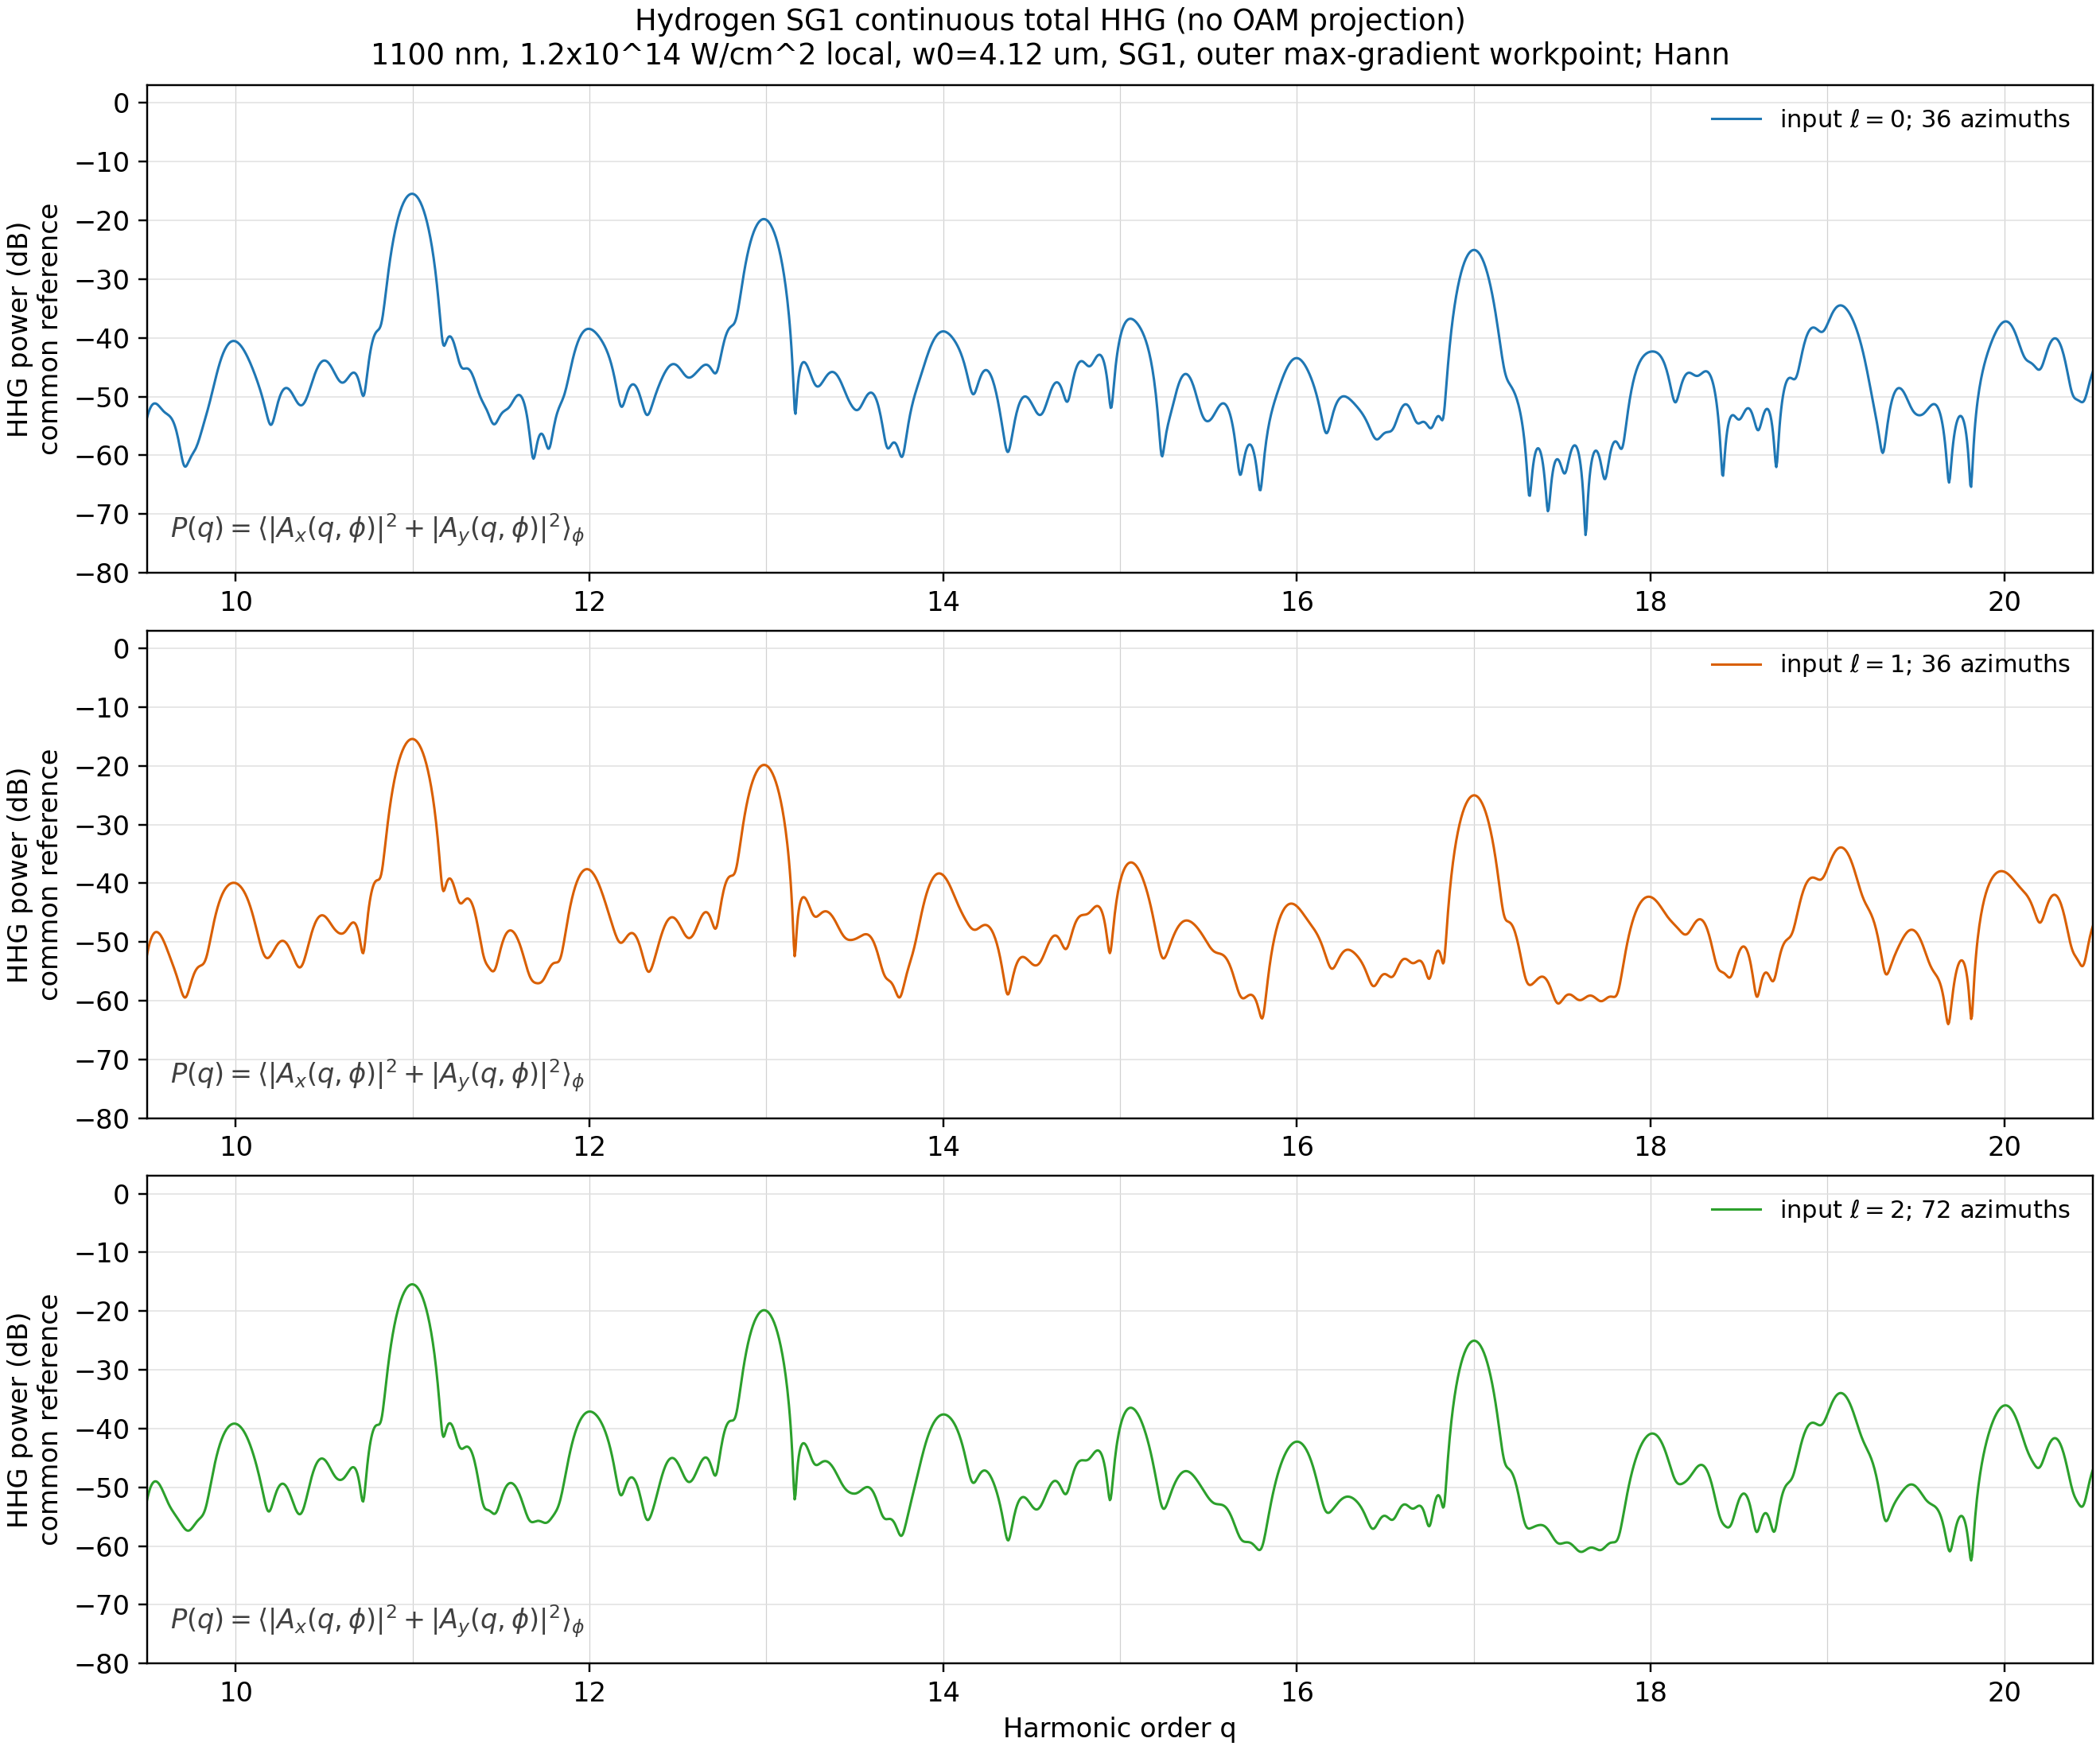
\includegraphics[width=0.8\linewidth]{reviewer_response_R1_figs/fig1_gas_hhg.png}
  \caption{氢原子 l=0,1,2 连续 HHG 谱（显示 10--20 阶）：高阶偶次通道依然
  清晰可见。显示范围远低于时间采样奈奎斯特上限
  （$\omega_{\mathrm{nyq}}/\omega_0 \approx 607$）。}
  \label{fig:gas_hhg}
\end{figure}

\begin{figure}[htbp]
  \centering
  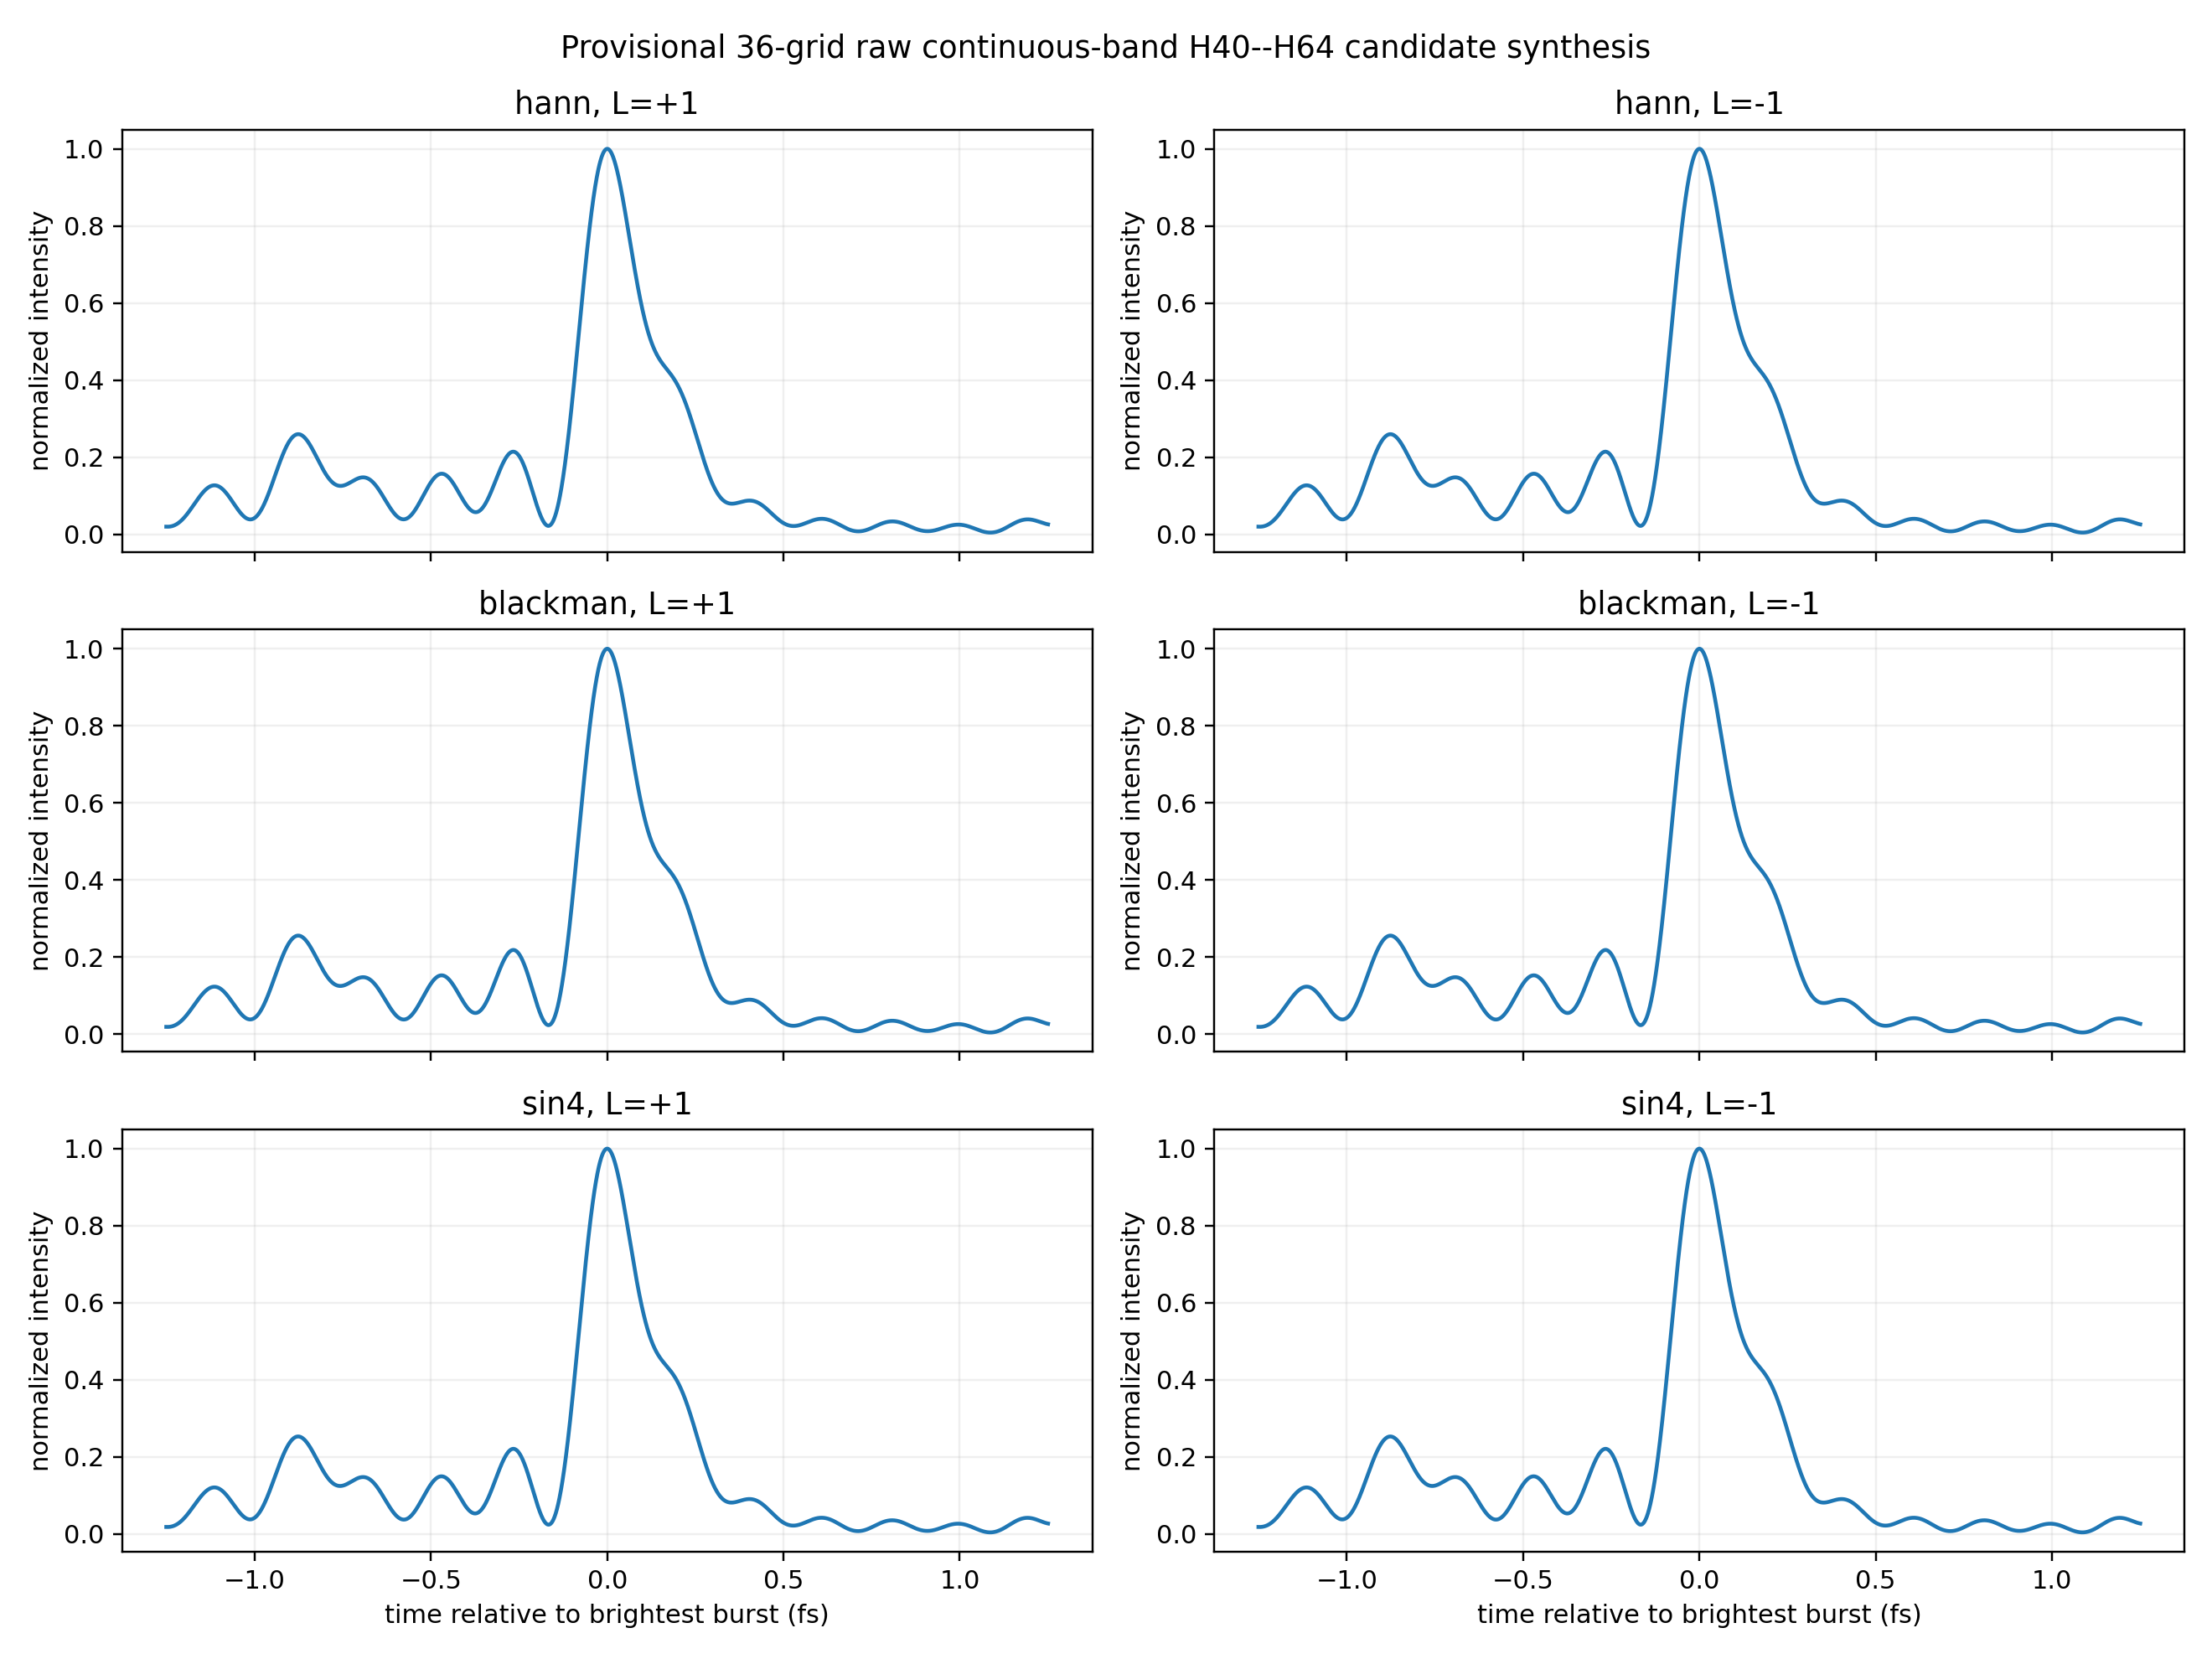
\includegraphics[width=0.8\linewidth]{reviewer_response_R1_figs/fig3_attosecond.png}
  \caption{由气体谐波合成的阿秒脉冲（连续阿秒脉冲单元），脉宽短于固体的
  对应结果。}
  \label{fig:attosecond}
\end{figure}

\section*{第 2 条 —— 径向与方位角梯度的各自作用；$\ell=0$ 的情形}

\reviewer{From the text one could infer that the $\pm1$ extra OAM appears only due
to the radial gradient of the field (``positioned at the radial location where the
transverse gradient of the vortex reaches its maximum'', ``for vortex beams,
$G_r$ increases with decreasing beam waist and increasing super-Gaussian order
$N$''), in a way that it is not connected to the azimuthal variation. It would be
interesting to gain more insight about the individual roles of the radial and
azimuthal field variations. In addition, the reason why there is no effect if the
beam does not carry OAM is not clear, as equation (1) for $\ell=0$ contradicts the
need of using a vortex beam (there is still a radial field gradient if the there is
no OAM). Is it because the OAM is needed to break the symmetry in centrosymmetric
systems and allow the generation of even harmonics and once this condition is
fulfilled the magnitude of the even harmonics depends also in the radial field
variation?}

\response 感谢审稿人指出这一点，它暴露了我们表述上的欠妥之处。分两部分回答。

\medskip\noindent\textbf{(i) 径向与方位角梯度的各自作用。}
我们把场梯度分解为径向分量和方位角分量，保持其余参数完全不变、分别演化。
结果表明（新图 \ref{fig:radial_azimuthal}）：偶次谐波的梯度通道几乎完全来自
\textbf{径向}梯度，方位角贡献可以忽略。这一点现已在正文中明确写出。

\begin{figure}[htbp]
  \centering
  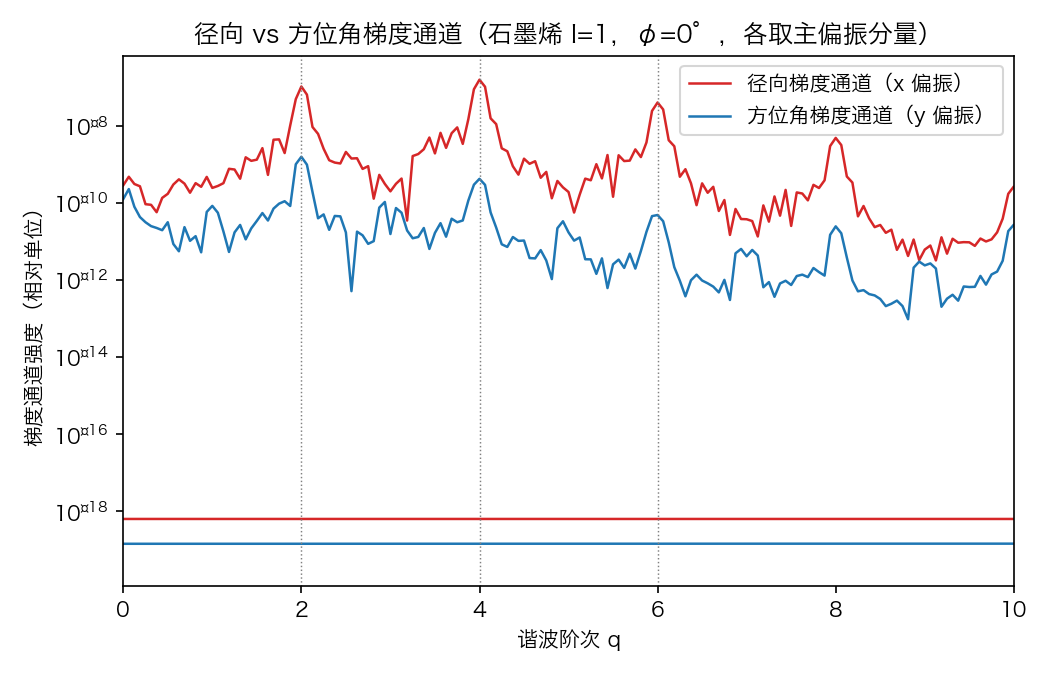
\includegraphics[width=0.75\linewidth]{reviewer_response_R1_figs/fig5_radial_vs_azimuthal.png}
  \caption{径向梯度通道（x 偏振）与方位角梯度通道（y 偏振）的 HHG 谱对比
  （石墨烯 l=1，$\varphi=0^\circ$，各取主偏振分量）：径向梯度比方位角强约两个
  数量级。参数：两带石墨烯（$\gamma_0=2.7$ eV）、SGV5、$w_0=3\,\mu$m、
  $\lambda=2400$ nm、$I=0.1$ TW/cm$^2$、$\mu=0.2583$ eV、300 K、T2=10 fs、
  平滑 4+8+4 共 16 周期、k200$\times$200/q240、dt=0.1、stride=5、
  continuous\_shifted\_bz、fused\_observable\_sync；梯度分量分别取
  radial\_only 与 azimuthal\_only。}
  \label{fig:radial_azimuthal}
\end{figure}

\medskip\noindent\textbf{(ii) $\ell=0$ 的情形。}
我们原先的说法是思维惯性所致：想当然地认为``不输入 OAM 就不会输出 OAM''。
审稿人说得对：方程 (1) 在 $\ell=0$ 时依然预言偶次谐波 $L=\pm1$，纯径向梯度
（无 OAM）就应该足够。我们完成了 $\ell=0$ 的计算，预言得到证实：
\textbf{非涡旋光束的偶次谐波依然携带 $L=\pm1$}，奇次谐波为 $L=0=q\ell$
（新图 \ref{fig:l0_conventions}）。

这带来重要的远场推论：奇次谐波（$L=0$）集中在轴附近、发散小；偶次谐波形成
外环（$L=\pm1$）、发散角更大。实验上这意味着——\textbf{产生 XUV 涡旋不再需要
驱动光携带 OAM，只需要强径向梯度}。强梯度（紧聚焦/结构化）驱动场已有大量
工作，且不需要 OAM 输入意味着驱动光的光束质量问题不再构成限制；氢原子在温和
参数下已得到不错的结果，本工作的工程可行性很高。

若需要单手性外环通道（如 $L=+1$），有两条可行的实验路线：(a) XUV 圆偏振片
（四分之一波延迟器加线偏振分析器）直接选出径向偏振偶次谐波的一个旋性通道；
(b) 叉形光栅加 $m=\pm1$ 端口与中心光阑，分离两个旋性分量并恢复单手性
$L=1$ XUV 涡旋。两个方案都已在修改稿中讨论。

\begin{figure}[htbp]
  \centering
  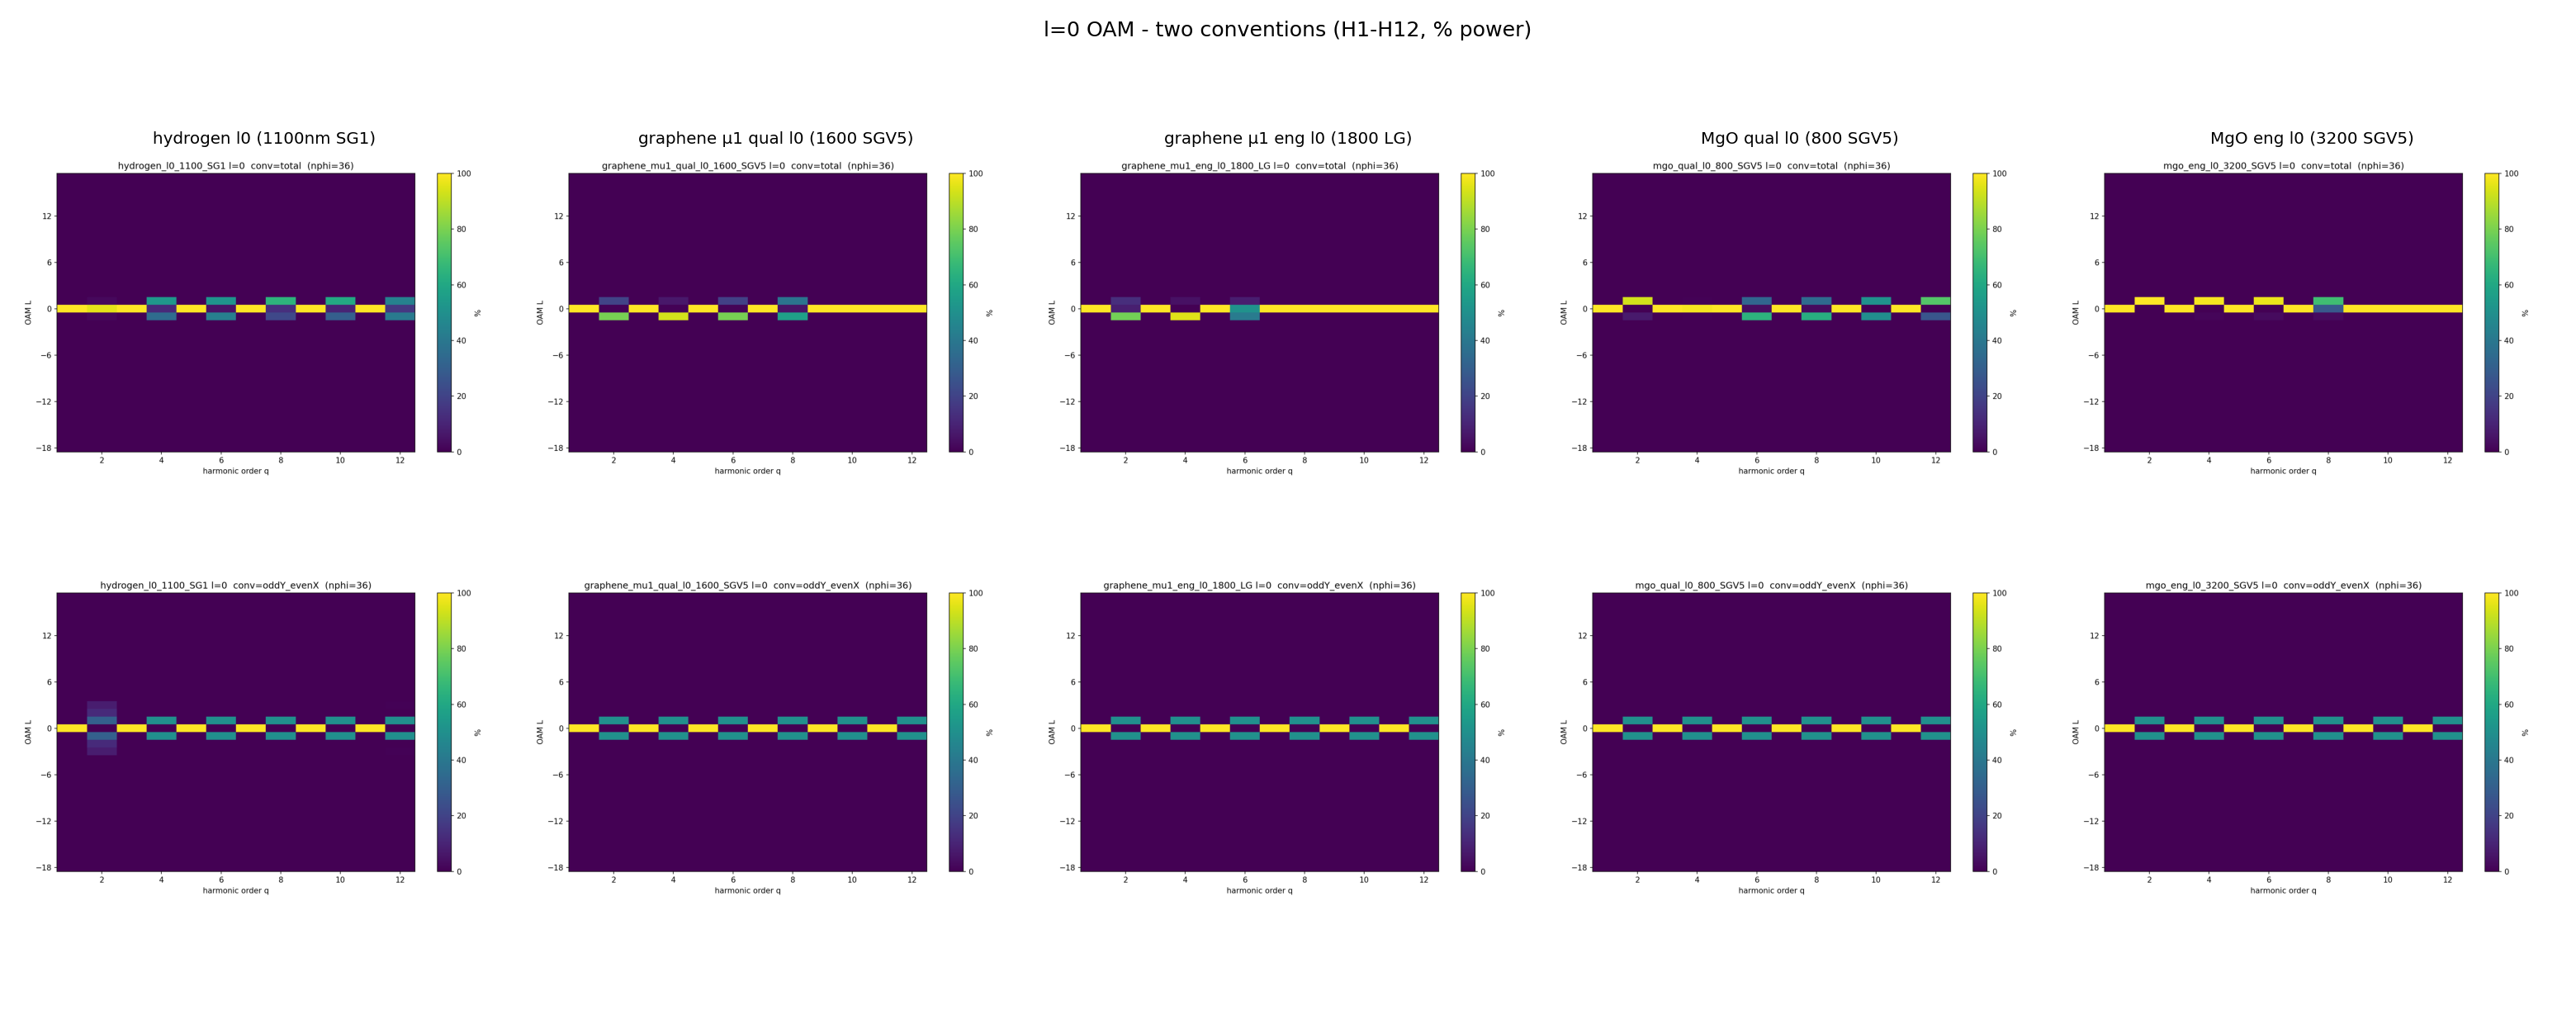
\includegraphics[width=0.98\linewidth]{reviewer_response_R1_figs/fig4_l0_two_conventions.png}
  \caption{五种体系 l=0 的 OAM 分析（两种惯例）：偶次谐波携带 $L=\pm1$，
  无需 OAM 输入。}
  \label{fig:l0_conventions}
\end{figure}

\section*{第 3 条 —— 图 1 中``偶极近似''的标注}

\reviewer{In connection with the previous point, it is not clear to me why the
non-vortex case is denoted as ``dipole approximation'' in Fig.1 (blue curve). I
would expect this label for the case of the vortex beam with no gradient effects
(red curve). And does the non-vortex case still account for the radial field
variation?}

\response 抱歉，这是我们标注不清造成的描述疏忽；我们已修改图 1 及其图注。
需要说明的是，图 1 三条曲线比较的是\textbf{垂直偏振（$x$）通道}的偶次谐波，
即 OAM 分析（偶次取 $x$ 分量）所使用的通道。三条曲线对应：

\begin{itemize}
  \item \textbf{蓝线}——空间均匀场、无 OAM 输入：无偶次谐波（符合预期）。
  \item \textbf{红线}——空间均匀场、\textbf{但保留 $\ell=1$ 的 OAM 相位}：
  依然无偶次谐波。这条曲线回答的问题是：单独的方位角相位梯度能否产生偶次
  谐波？已有文献讨论过该机制（如 Wang \& Cheng, \emph{J.\ Phys.\ B}），而我们的
  结果显示在我们的构型下不能。
  \item \textbf{黑线}——完整场（径向梯度与 OAM 兼有）：出现偶次谐波。
\end{itemize}

这个对比说明：我们工作中偶次谐波的 $x$（垂直）通道——即 OAM 分析所用的通道
——完全来自\textbf{径向}场梯度，而不是已有研究中的方位角相位梯度。据我们所知，
这一径向梯度机制此前未被识别过。图 1 的标注已相应修正。

\section*{第 4 条 —— ``偶极近似''术语与 $\exp(-i\ell\varphi)$ 依赖}

\reviewer{The description of the OAM rule in the dipole approximation seems
confusing: the $\exp(-i\ell\varphi)$ dependency of the electric field appears
beyond the dipole approximation. Even though the mathematical derivations make
sense, the terminology could be clarified and put into context with respect to
the literature.}

\response 同意，这个术语是我们表述上的疏忽，已在修改稿中澄清：光束的
$\ell$ 依赖相位是驱动场的\textbf{空间结构}属性，它通过场的空间依赖进入严格偶极
近似之外的物理。我们现在明确区分两个概念——光与物质相互作用中的``偶极近似''
（场无空间变化）与``光束空间结构''（携带 $\exp(-i\ell\varphi)$ 相位）——并把
推导与 OAM 选择定则的相关文献联系起来。

\section*{第 5 条 —— 紧聚焦下的纵向场分量}

\reviewer{The employed driving field has a very strong longitudinal component due
to tight focusing (comparable to the transversal field for the field parameters
used in the manuscript) [M. Lax et al. Phys. Rev. A 11, 1365]. Is the effect of
this component taken into account? Also, the presence of this longitudinal field
contradicts the sentence ``The driving electric field lies in the plane of the
nanoflake, with its polarization direction indicated in the figure'' in the text.}

\response 这是很重要的一点，我们用一个专门的三维研究处理了它。我们建立了
八带多轨道石墨烯模型（每个格点 $(s,p_x,p_y,p_z)$，Slater--Koster 参数），驱动场
为完整的 Maxwell 投影矢量场 $(A_x,A_y,A_z)$，包含纵向分量与完整的 $3\times3$
场梯度张量，从而显式保留 $E_z$ 耦合和纵向磁力 $\mathbf{J}\times\mathbf{B}$
（新图 \ref{fig:3d_validation}）。结论如下：

\begin{itemize}
  \item $E_z$ 介导的 $\pi$--$\sigma$ 耦合真实存在，但对稿件所报告的面内 HHG
  观测量可以忽略：所考虑的谐波（H2--H8）全部低于 $\pi\to\sigma^*$ 阈值
  （$\approx 8.3$ eV），$E_z$ 只能驱动虚的面外极化；纵向极化电流比面内电流弱
  $4$--$5$ 个数量级。
  \item 由 $z\to-z$ 镜像对称性，面内观测量在 $A_z\to-A_z$ 下是偶的，因此
  $E_z$ 对面内 HHG 的修正是二阶小量。
  \item 磁力 $|\mathbf{J}\times\mathbf{B}|$ 受非相对论 $v/c$ 因子抑制
  （相对电场力约 $10^{-5}$）。
  \item 我们还在\textbf{稿件所用的精确参数}（$\mu=1$ eV、高斯 8 周期、无 T2、
  1600 nm、0.25 TW/cm$^2$）下验证了这些结论，结论不变。
\end{itemize}

``驱动电场位于纳米片平面内''这句话已修正：现在指占主导的横向分量，纵向分量的
作用（对所报告观测量定量可忽略）在新附录中明确讨论。

\begin{figure}[htbp]
  \centering
  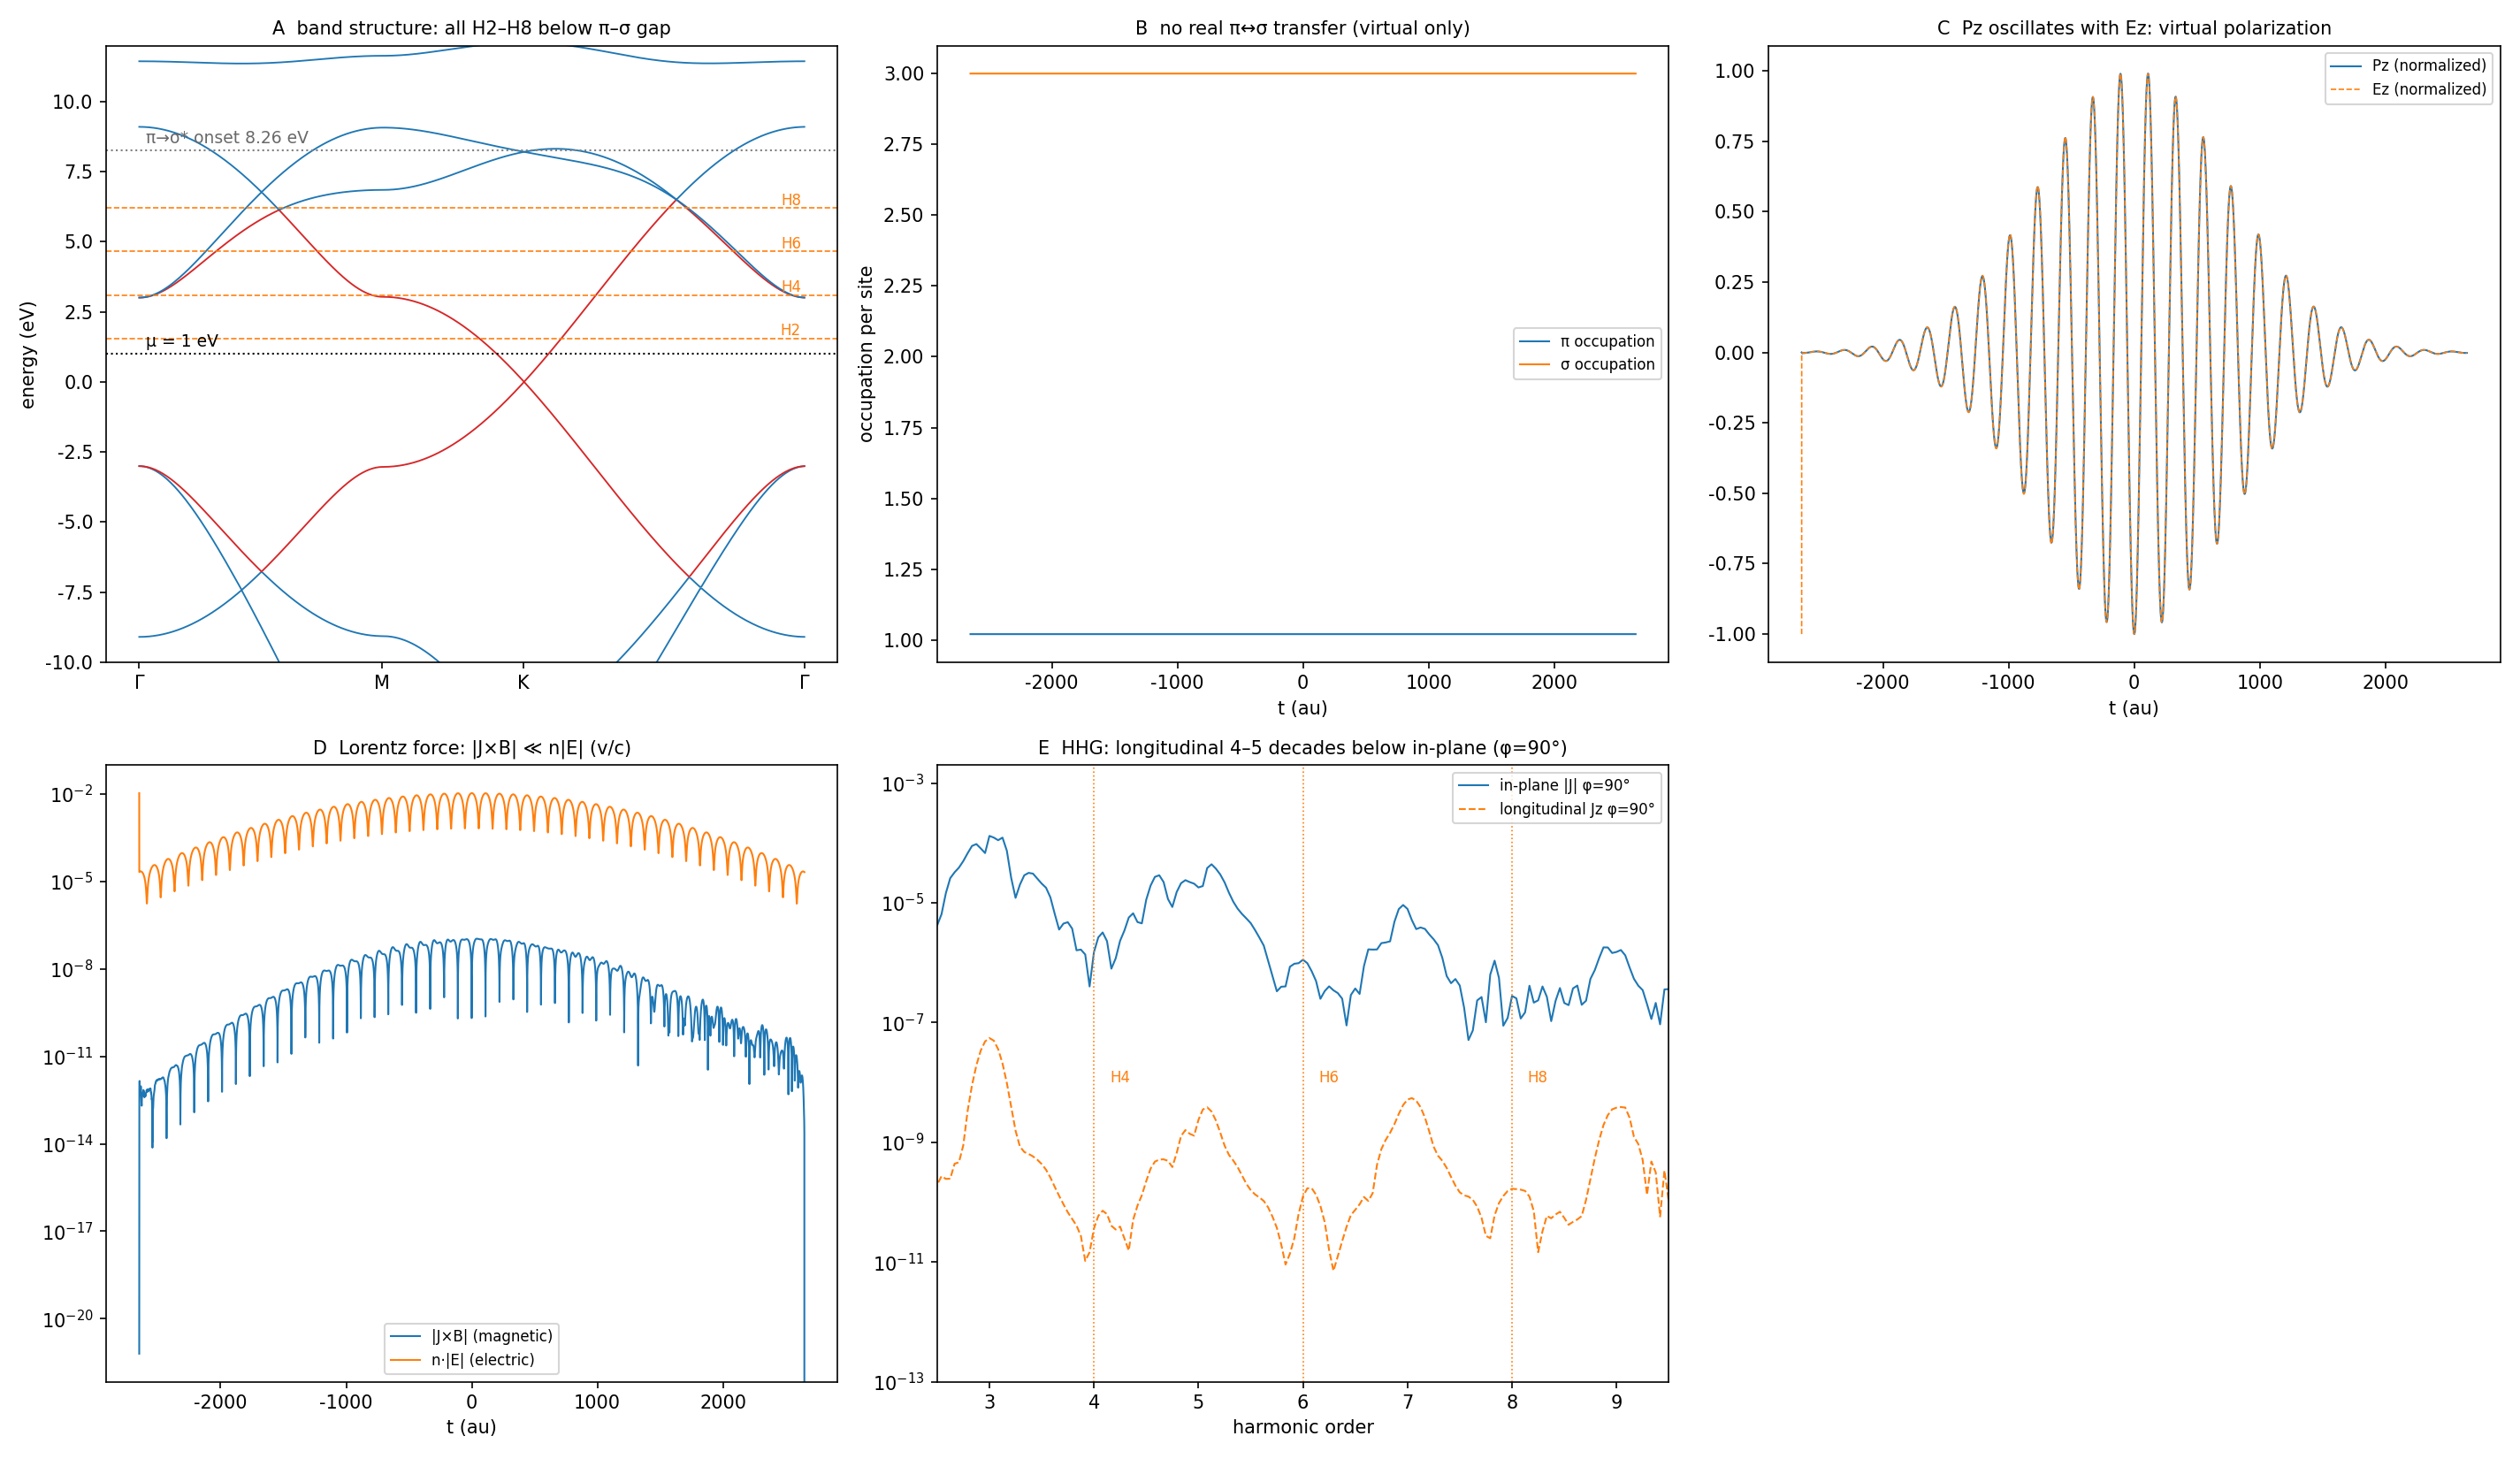
\includegraphics[width=0.98\linewidth]{reviewer_response_R1_figs/fig7_3d_validation.png}
  \caption{三维八带全矢量验证：能标（A）、虚极化（B--C）、$v/c$ 磁力压低
  （D）与纵向/面内谱对比（E，$\varphi=90^\circ$）。模型：八带
  $(s,p_x,p_y,p_z)\times(A,B)$、最近邻 Slater--Koster（Saito PRB 46,1804）、
  $s$--$p_z$ 偶极 0.5 \AA{}。光束 SGV5、l=1、$w_0=3\,\mu$m。全部面板：
  $\lambda=1600$ nm、$\mu=1$ eV、300 K、无 T2、高斯 8 周期、$I=0.25$
  TW/cm$^2$（local\_at\_workpoint）、nk=64、dt=0.1、full\_xyz、velocity
  gauge。}
  \label{fig:3d_validation}
\end{figure}

\section*{第 6 条 —— 既然梯度有影响，为何奇次谐波 100\% 是偶极？}

\reviewer{Why are the odd harmonics, such as the 5th harmonic, 100\% dipole if
there is a difference between the calculations with and without field gradients?
[See panel 1(a)]}

\response 我们把计算响应分解为两个分别演化的通道：\textbf{均匀通道}（空间均匀
场，标准偶极响应）与\textbf{梯度通道}（对场梯度的线性响应）。分解显示
（新图 \ref{fig:channels}）：

\begin{itemize}
  \item 均匀通道只贡献\textbf{奇次}谐波（$L=q\ell$）；
  \item 梯度通道贡献\textbf{偶次}谐波（$L=q\ell\pm1$），在奇次阶上可以忽略。
\end{itemize}

因此奇次谐波由偶极通道主导（梯度修正微乎其微），这解释了它们表现为``100\%
偶极''；而偶次谐波的存在完全归功于梯度通道。正文已明确说明。

\begin{figure}[htbp]
  \centering
  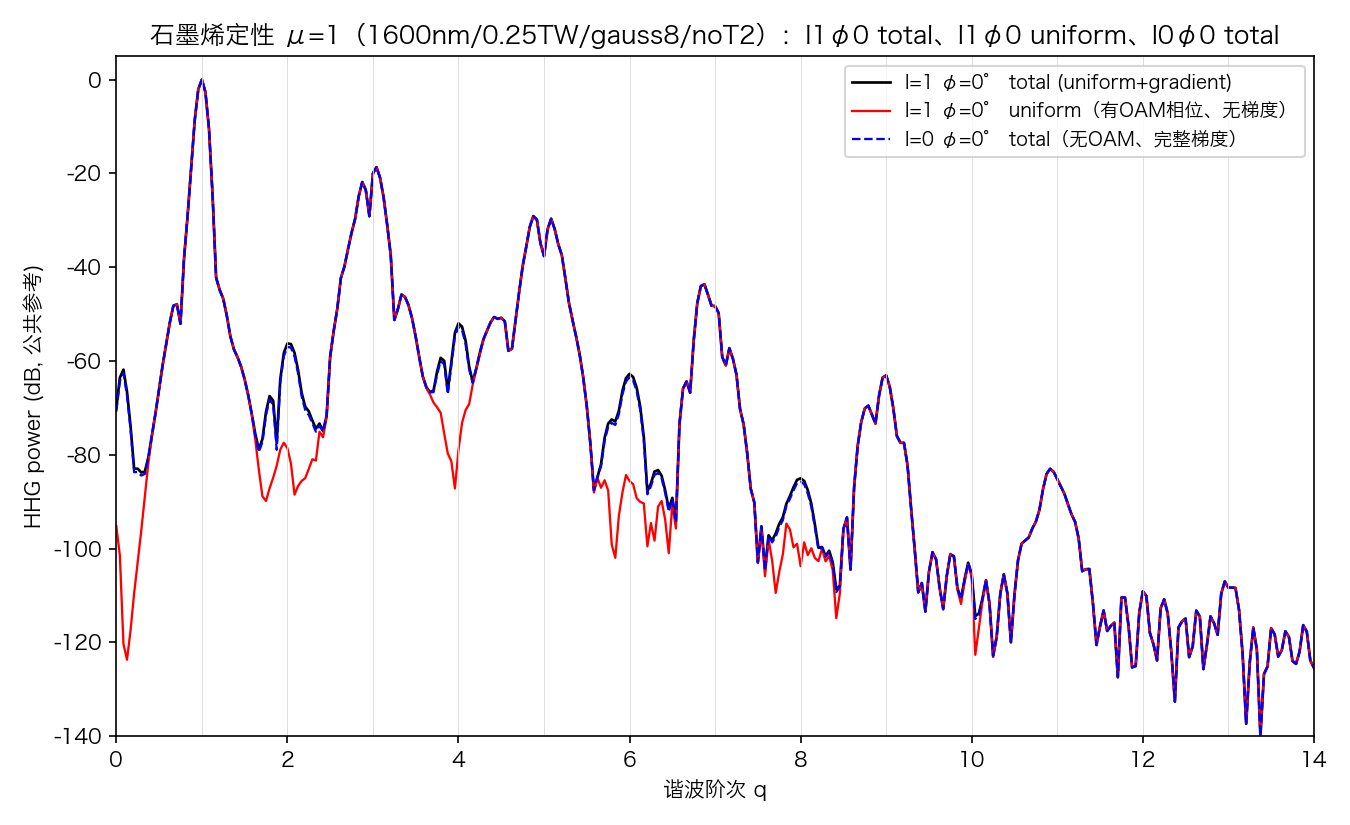
\includegraphics[width=0.8\linewidth]{reviewer_response_R1_figs/fig7_channels_user.png}
  \caption{石墨烯 l=0 的通道分解：均匀通道（y 偏振）贡献奇次谐波，梯度通道
  （x 偏振）贡献偶次谐波。参数：两带石墨烯、SGV5、$w_0=3\,\mu$m、
  $\lambda=1600$ nm、$r/w_0=0.98952$、$I=0.25$ TW/cm$^2$
  （local\_at\_workpoint）、$\mu=1$ eV、300 K、无 T2、高斯 8 周期、
  k200$\times$200/q240、dt=0.1、stride=1、full gradient、
  continuous\_shifted\_bz、fused\_rk2\_sync、$\varphi=0^\circ$。}
  \label{fig:channels}
\end{figure}

\section*{第 7 条 —— 更高谐波阶次}

\reviewer{Why do the figures only show the lower-order harmonics? Is it because
the approximation of the absence of magnetic contribution breaks for higher orders
as shown in the SM? I would be curious to know how the higher orders behave too.}

\response 主图只显示低阶的原因是\textbf{模型}的限制，而非物理的限制：在我们的
石墨烯两带模型中，偶次峰在第 6 阶之后不再清晰（能带结构限制了可及谐波范围）。
这正是我们为低阶选择该模型的原因。为回答审稿人对高阶的好奇，我们提供几组互补
的结果：

\begin{enumerate}
  \item 补充材料中的二维 Mathieu 模型在高阶依然清晰可见。
  \item 我们从严谨的块体出发，开发了半导体布洛赫方程（SBE）+ Peierls 桥，
  给出更清晰的石墨烯块体结论。
  \item 我们完成了完整的 144 角 OAM 分辨计算（xy 惯例：奇次用 $y$、偶次用
  $x$），覆盖石墨烯\textbf{工程与定性参数}以及 MgO\textbf{工程与定性参数}，
  选择定则（奇次 $L=q\ell$；偶次 $L=q\ell\pm1$）直到第 12 阶都干净成立
  （新图 \ref{fig:144_overview}）；hBN 定性参数亦满足 $L=q\ell$
  （新图 \ref{fig:hbn}）。
\end{enumerate}

\begin{figure}[htbp]
  \centering
  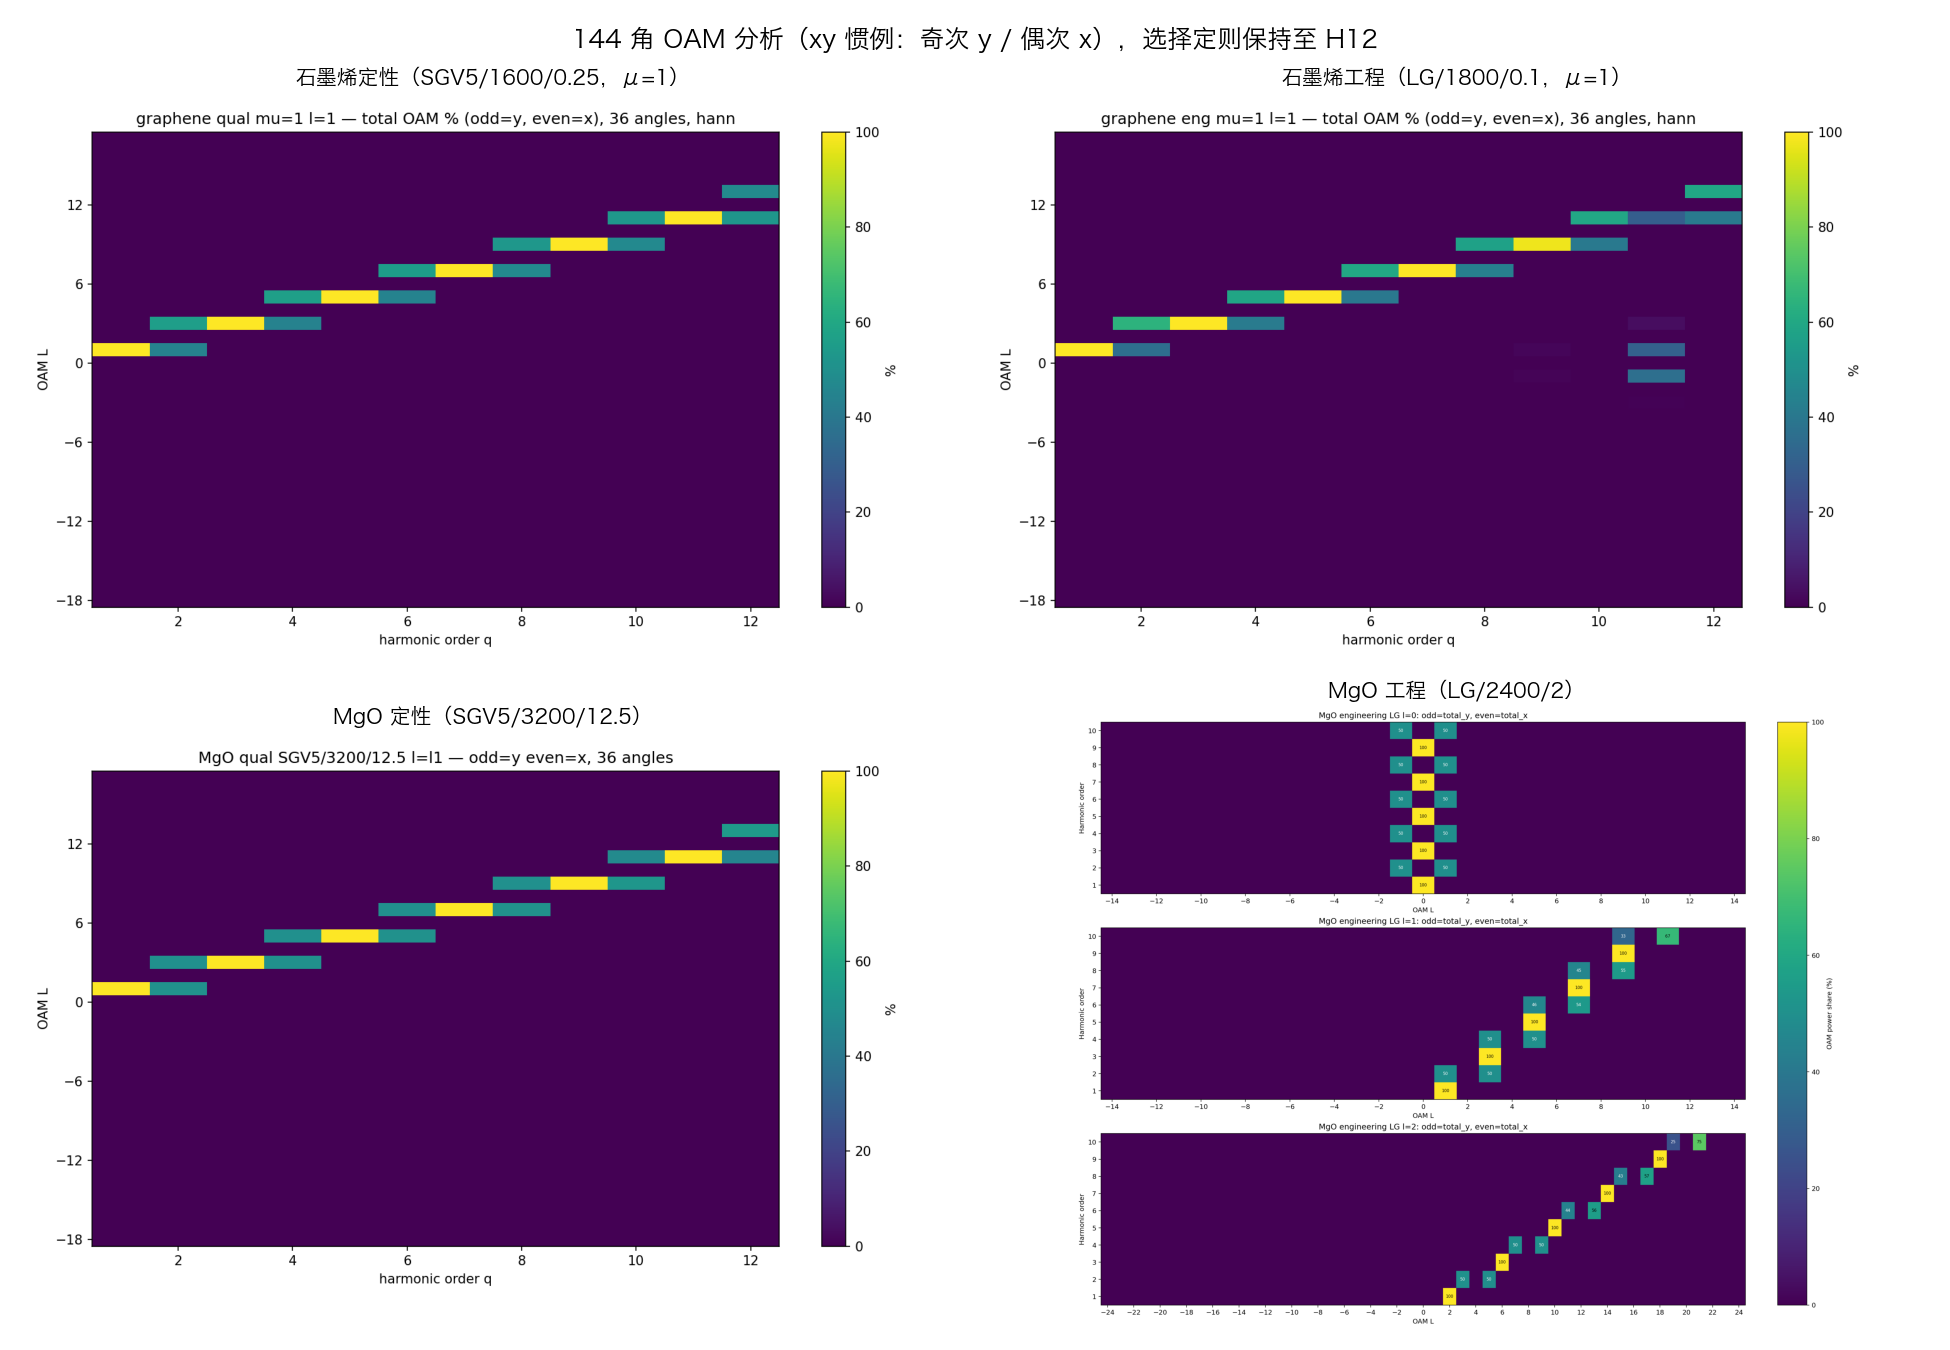
\includegraphics[width=0.98\linewidth]{reviewer_response_R1_figs/fig9_144_overview.png}
  \caption{石墨烯与 MgO 的 144 角 OAM 分析（工程/定性参数，xy 惯例）：
  选择定则保持至 H12。}
  \label{fig:144_overview}
\end{figure}

\begin{figure}[htbp]
  \centering
  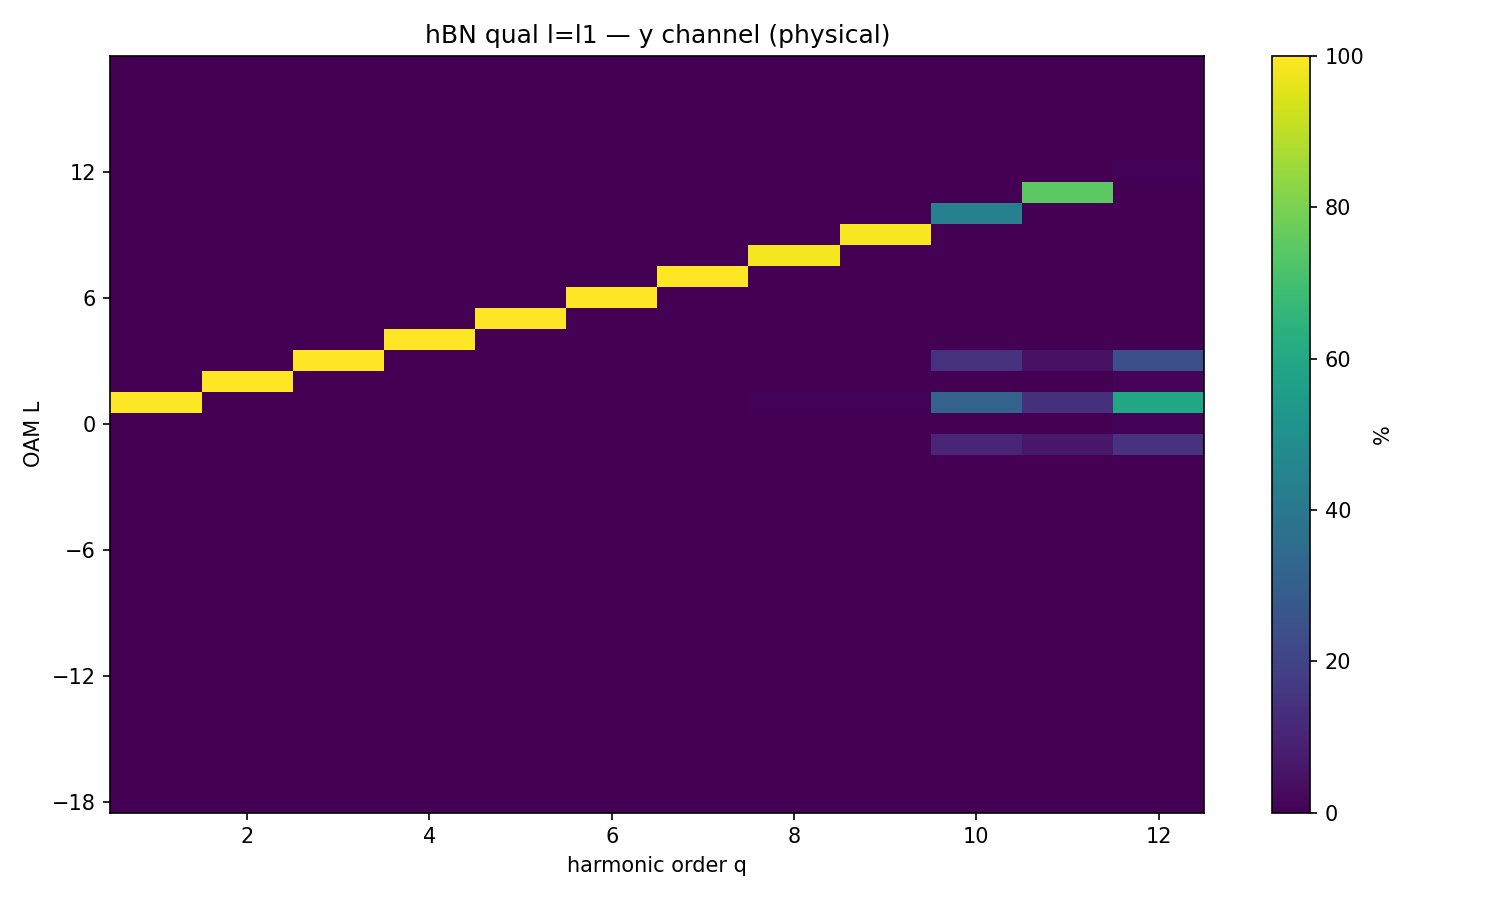
\includegraphics[width=0.7\linewidth]{reviewer_response_R1_figs/fig10_hbn_oam.png}
  \caption{hBN 定性（SGV5/1600/0.25，$\mu=0$）l=1 的 y 通道 OAM：
  $L=q\ell$，H1--H9 纯度大于 98\%。}
  \label{fig:hbn}
\end{figure}

\section*{第 8 条 —— 参考文献位置}

\reviewer{It seems that some references in the introduction could be misplaced,
in particular [7-12] and [18].}

\response 感谢审稿人指出。我们重新检查了引言中所有引用的位置，修正了
[7--12] 与 [18] 的错放，并重新核对了其余引用。

\section*{第 9 条 —— 与电子跃迁 OAM 选择定则的区别}

\reviewer{The derivation of the OAM selection rules from the commutation relations
seems original and accurate. On the other hand, the interaction of vortex beams
with matter leads to well-known selection rules for electronic transitions
[Examples: Pic\'on A. et al. New J. Phys. 12 083053 (2010); Duan, Y. et al
J. Phys. B: At. Mol. Opt. Phys. 52 184002 (2019)]. The transition OAM selection
rules have a different nature than those studied in the present manuscript, so it
could be helpful for a potential reader to mention this distinction.}

\response 同意，感谢审稿人的建议。我们在修改稿中加了一段，明确区分：

\begin{itemize}
  \item \textbf{电子跃迁 OAM 选择定则}（Pic\'on 等、Duan 等）：约束单次
  光--物质跃迁中转移的 OAM（如光电离或共振跃迁中的 $\Delta m=\pm1$）；
  \item 本工作推导的\textbf{谐波 OAM 选择定则}：描述所发射谐波的 OAM 含量
  （$L=q\ell$ 与 $L=q\ell\pm1$），是发射场的集体宏观性质。
\end{itemize}

两者性质不同，我们已明确说明并给出相应引用，便于读者理解这一区别。

\section*{第 10 条 —— 非共线构型中的 OAM 分辨 XUV 探测}

\reviewer{The authors state that ``The coexistence and controllable separation of
multiple OAM channels at the same harmonic order provides a route toward OAM
resolved XUV detection, where angular-momentum components are mapped onto spatial
coordinates''. This has been widely done in noncollinear configurations
[G. Gariepy, et al. Phys. Rev. Lett. 113, 153901 (2014); F. Kong, et al,
Nat. Commun. 8, 14970 (2017); D. Gauthier, et al, Nat. Commun. 8, 14971 (2017).]}

\response 感谢审稿人指出这些工作，我们此前并不了解这一脉络。我们已修改相应
句子并引用 Gariepy 等、Kong 等和 Gauthier 等，承认 OAM 分量的空间映射已在
非共线构型中得到演示。同时我们把表述收敛到本工作的\textbf{共线}方案：在同一
谐波阶次上多个 OAM 通道的共存是选择定则本身带来的固有性质。

\section*{修改清单}

\begin{enumerate}[label=\arabic*.]
  \item 新增气体章节：氢原子（SG1、1100 nm）中得到相同选择定则；无需双靶材
  干涉偶次即干净；阿秒脉冲合成脉宽更短（图 \ref{fig:gas_oam}、
  \ref{fig:gas_hhg}、\ref{fig:attosecond}）。
  \item 新增 $\ell=0$ 结果：非涡旋光束的偶次谐波携带 $L=\pm1$；远场推论
  （内圈奇次/外圈偶次环）与两条单手性 XUV 涡旋实验方案（圆偏振片；叉形光栅
  $+$ $m=\pm1$ 端口 $+$ 光阑）。
  \item 径向/方位角梯度分解，证明偶次谐波由径向梯度驱动（图 \ref{fig:radial_azimuthal}）。
  \item 修正图 1 标注与术语（偶极近似 vs 光束空间结构）。
  \item 新附录：三维八带模型 $+$ Maxwell 投影矢量场；$E_z$ 与纵向磁力可忽略
  （4--5 个数量级），并在稿件参数下验证（图 \ref{fig:3d_validation}）。
  \item 均匀/梯度通道分解，解释奇次为何是偶极主导（图 \ref{fig:channels}）。
  \item 高阶行为：二维 Mathieu（补充材料）、SBE+Peierls 块体桥、石墨烯与 MgO
  工程/定性参数 144 角 OAM 直到 H12（图 \ref{fig:144_overview}）、hBN 定性
  （图 \ref{fig:hbn}）。
  \item 参考文献 [7--12]、[18] 重新定位；新增引用（Pic\'on 2010、Duan 2019、
  Gariepy 2014、Kong 2017、Gauthier 2017、Wang \& Cheng, \emph{J.\ Phys.\ B}）。
\end{enumerate}

\end{document}
